\documentclass{standalone}
\begin{document}
\markboth{CHAPTER 1. MATERIALS AND METHODS}{1.5. PCA}
\section{Principal Component Analysis}
Principal component analysis (PCA) is a technique to reduce data dimensionality.
It replaces the $n$ original variables by a smaller number, $q$, of linear combinations, called principal components, of the original variables.
The application areas include data compression, image analysis, pattern recognition, regression and classification prediction\cite{PCA}.\\
The most common definition of PCA, due to Hotelling, states that for a set of observed data vectors 
$ \{ \mathbf{t}_{n} \}$, $n \in \{1, \dots, N \} $, the $q$ principal axes $\mathbf{w}_j$, $j \in \{ 1, \dots, q \} $ are those orthonormal axes onto which the retained variance under projection is maximal.
The vectors $\mathbf{w}_j$ are given by the $q$ dominant eigenvectors (i.e. those with the largest associated eigenvalues $\lambda$) of the sample covariance matrix $\mathbf{S} = \sum_{n}^{} ( \mathbf{t_n} - \mathbf{\bar{t}}) ( \mathbf{t_n} - \mathbf{\bar{t}})^T / N$ such that  $ \mathbf{S}\mathbf{w}_j = \lambda_j \mathbf{w_j}$ and where $\mathbf{\bar{t}}$ is the sample mean.
The vector $\mathbf{x}_{n} = \mathbf{W^T} (\mathbf{t_n} - \mathbf{\bar{t}})$, where $ \mathbf{W} = (\mathbf{w}_1 , \mathbf{w}_2 \dots \mathbf{w}_j)$ is thus a q-dimensional reduced representation of the observed vector $\mathbf{t}_{n}$ \cite{PCA}.
As we have mentioned, $\lambda_j$ is just the variance of each new feature dimension.
How to choose an appropriate $q$ depends on the Variance Contribution Rate  $\alpha_j = \lambda_j / \sum_{j}^{} \lambda_j $. 
This can be determined by looking at the cumulative explained variance ratio as a function of the number of components as shown in figure \ref{cumulativevr}.


\begin{figure}[ht]

    \centering
    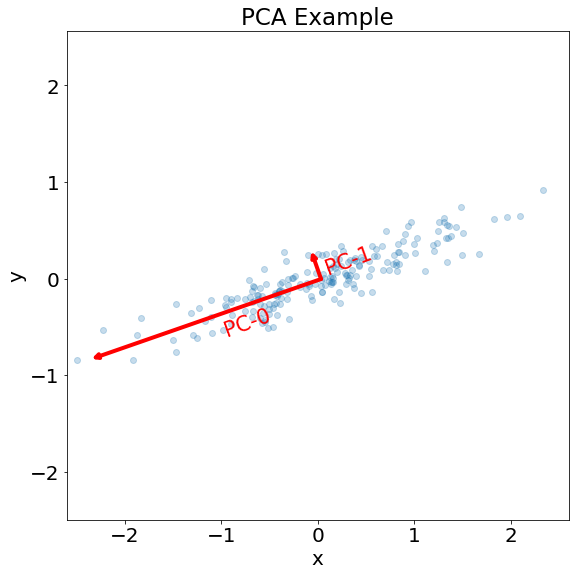
\includegraphics[width=0.62\textwidth]{../images/PCAexample1.png}
    
    \caption{Example of Principal Component Analysis.
     The red vectors represent the principal axes of the data, and the length of the vector is an indication of the variance of the data when projected onto that axis.}
    \label{PCAexample}
    
    \end{figure}

\markboth{CHAPTER 1. MATERIALS AND METHODS}{1.5. PCA}

\begin{figure}[htp]

    \centering
    \includegraphics[width=.68\textwidth]{../images/cumulative3.png}
    
    \caption{Example of cumulative explained variance ratio as a function of the number of components. This curve quantifies how much of the total variance is contained within the first N components. We can see that the first 10 components contain approximately $75 \%$ of the total variance, while to the reach the $100 \%$ you need around 50 components.}
    \label{cumulativevr}
    
    \end{figure}

\end{document}